\documentclass[12pt, a4paper,twoside]{tesi_upf}

%CODIFICATION
\usepackage[latin1]{inputenc}
%LENGUAGE
\usepackage[catalan,english]{babel}
%ONLY TO OBTAIN MARK BANK INDEX INDICATION A4
\usepackage[cam,a4,center,frame]{crop}
%INCLUDE GRAPHICS AND THE LOGO OF THE UPF
\usepackage{graphicx}
%FONTS TIMES OR GARAMOND, 
\usepackage{times}
%\usepackage{garamond}
%WITHOUT HEADINGS: NO MODIFICATION
\pagestyle{plain}
%FOR THE INDEX OF SUBJECTS
\usepackage{makeidx}
\makeindex
%BIBLIOGRAPHY STYLE
\bibliographystyle{apalike}
%SELECT LANGUAGE
\selectlanguage{catalan}

% Equations
\usepackage{amsmath,amssymb,amsfonts}

% Hyperreferences
\usepackage{url}
%\usepackage{hyperref}

\hyphenation{Re-use}

%THE TABLE OF CONTENTS IS TITLE CONTENTS
%\addto\captionscatalan
\renewcommand{\contentsname}{\Large \sffamily Table of contents}

%ADD YOUR DATA
\title{Enabling Spatial Reuse in Future Wireless Local Area Networks:\\ a Machine Learning \& Game Theoretic Proposal}
%\subtitle{The subtitle of the thesis: Required}
\author{Francesc Wilhelmi Roca}
\thyear{2020}
\department{of Information and Communication Technologies}
\supervisor{Boris Bellalta, Cristina Cano \& Anders Jonsson}

\begin{document}

\frontmatter
\maketitle
\cleardoublepage

%%%%%% Dedication
\noindent Write here your dedication
\cleardoublepage
%%%%%% End dedication

%%%%%% Thanks
\noindent {\Large \sffamily Acknowledgments} 
\cleardoublepage
%%%%%% End of thanks

%ABSTRACT IN TWO LEGUAGES.
\selectlanguage{english}
\section*{\Large \sffamily Abstract}
The Spatial Reuse (SR) operation is gaining momentum in the newest IEEE 802.11 family of standards due to the overwhelming requirements posed by next-generation wireless networks. In particular, the increasing traffic capacity and number of concurrent devices compromise the efficiency of Wireless Local Area Networks (WLANs) and throw into question their decentralized nature. The SR operation, initially introduced by the IEEE 802.11ax-2020/21 amendment and further studied in IEEE 802.11be-2024, is aimed at increasing the number of concurrent transmissions in an Overlapping Basic Service Set (OBSS), thus improving spectral efficiency. 

The SR operation has been initially defined as a distributed mechanism, but it is evolving towards coordinated schemes. Nevertheless, coordination entails communication and synchronization procedures that have not been defined yet. The necessary overhead to carry out coordination has implications on the performance of WLANs and remains unknown. Moreover, the coordinated scheme is not compatible with IEEE 802.11 devices not implementing it.

Given the SR-related problems faced by future WLAN deployments, Artificial Intelligence (AI) emerges as a promising solution able to overcome the challenges arisen from the complex and varying spatial interactions among devices. In particular, due to the challenges posed by coordination, in this thesis, we study the feasibility of Reinforcement Learning (RL)-based methods to overcome the SR problem in a decentralized manner.

... \textcolor{red}{[TO BE COMPLETED]}

\pagebreak
\selectlanguage{english}
\vspace*{\fill}
\section*{\Large \sffamily  Resum}

\vspace*{\fill}

\cleardoublepage
%END OF ABSTRACT

\section*{\Large \sffamily List of Publications}

\begin{enumerate}
	\item Wilhelmi, F., Mu�oz, S. B., Cano, C., Selinis, I., \& Bellalta, B. (2019). \textit{Spatial Reuse in IEEE 802.11 ax WLANs.} arXiv preprint arXiv:1907.04141.
	\item Wilhelmi, F., Barrachina-Mu�oz, S., \& Bellalta, B. (2019, October). \textit{On the Performance of the Spatial Reuse Operation in IEEE 802.11 ax WLANs.} In 2019 IEEE Conference on Standards for Communications and Networking (CSCN) (pp. 1-6). IEEE.
	\item Wilhelmi, F., Bellalta, B., Cano, C., \& Jonsson, A. (2017, October). \textit{Implications of decentralized Q-learning resource allocation in wireless networks}. In 2017 ieee 28th annual international symposium on personal, indoor, and mobile radio communications (pimrc) (pp. 1-5). IEEE.
	\item Wilhelmi, F., Cano, C., Neu, G., Bellalta, B., Jonsson, A., \& Barrachina-Mu�oz, S. (2019). \textit{Collaborative spatial reuse in wireless networks via selfish multi-armed bandits.} Ad Hoc Networks, 88, 129-141.
	\item Wilhelmi Roca, F., Barrachina Mu�oz, S., Bellalta, B., Cano Sand�n, C., Jonsson, A., \& Neu, G. (2019). \textit{Potential and pitfalls of multi-armed bandits for decentralized spatial reuse in WLANs.} Journal of Network and Computer Applications, 2019, 127.
	\item Barrachina-Mu�oz, S., Wilhelmi, F., Selinis, I., \& Bellalta, B. (2019, April). \textit{Komondor: a wireless network simulator for next-generation high-density WLANs.} In 2019 Wireless Days (WD) (pp. 1-8). IEEE.
	\item Wilhelmi, F., Barrachina-Munoz, S., Bellalta, B., Cano, C., Jonsson, A., \& Ram, V. (2020). \textit{A Flexible Machine-Learning-Aware Architecture for Future WLANs. IEEE Communications Magazine, 58(3), 25-31.}	
	\item Wilhelmi, F., Carrascosa, M., Cano, C., Ram, V., \& Bellalta, B. (2020). \textit{Usage of Network Simulators in Machine-Learning-Assisted 5G/6G Networks.}
\end{enumerate}
%Decentralized learning with cost in IEEE 802.11 WLANs
%Survey MABs for communications

%%PREFACE. 
%{\bf Preface}

\cleardoublepage
%END OF PREFACE

%TABLE OF CONTENTS: REQUIRED
\tableofcontents

%lIST OF FIGURES; ONLY IF THERE ARE FIGURES
%\listoffigures
%TO APPER THE LIST OF FIGURES IN THE TABLE OF CONTENTS 
%\addcontentsline{toc}{chapter}{List of figures}

%LIST OF TABLES; ONLY IF THERE ARE TABLES
%\listoftables
%TO APPEAR THE LIST OF TABLES IN THE TABLE OF CONTENTS
%\addcontentsline{toc}{chapter}{List of tables}

%START THE TEXT
\mainmatter

%%%%%%%%%%%%%%%%%
% INTRODUCTION
%%%%%%%%%%%%%%%%%
\chapter{Introduction}

% Introduction to IEEE 802.11 WLANs 
The Institute of Electrical and Electronics Engineers (IEEE) 802.11 family of protocols for wireless local area networks (WLANs) was first released in 1997 as a novel solution for physical (PHY) and medium access control (MAC) layers. Since that date, the standard has evolved to sustain the increasingly user requirements in terms of capacity, load, and coverage, as well as to serve for different purposes (e.g., mesh networking, security-enhanced communications, channel measurement, etc.). The set of novel and improved capabilities have been captured along the time in the plethora of amendments that followed the initial 802.11-1997 standard (e.g., 802.11b, 802.11g, 802.11h, etc.). 

% Next-generation of IEEE 802.11 WLAN standards
Looking forward, the next generation of WLAN standards is expected to revolutionize the telecommunications and converge along with 5G systems and beyond to expand to multiple domains, such as light communications (IEEE 802.11bb), Internet of Things (IEEE 802.11ah), vehicle-to-everything (IEEE 802.11bd), or next-generation positioning (IEEE 802.11az).%, or next-generation 60 GHz (IEEE 802.11ay).

One of the most influential amendments is the IEEE 802.11ax-2021 (11ax) amendment for High Efficiency (HE) WLANs \cite{bellalta2016ieee, deng2014ieee, khorov2018tutorial}, which primary goal is to enhance network efficiency in ultra-dense deployments, thus providing high capacity (up to 10 Gbps). The 11ax (commercially known as WiFi 6) includes a set of unprecedented techniques, such as Orthogonal Frequency Division Multiple Access (OFDMA), Downlink/Uplink Multi-User Multiple-Input-Multiple-Output (DL/UL MU-MIMO), and Spatial Reuse (SR), to address the broad range of issues arisen from high-density scenarios \cite{merlin2015tgax}.

% What is SR and what it is aimed to solve
This thesis focuses on the SR operation that was initially conceived for IEEE 802.11ax WLANs and that is now evolving in the IEEE 802.11be. SR is meant to enhance spectral efficiency by increasing the number of parallel transmissions in high-dense deployments. To this end, SR proposes a mechanism to improve the probability of ignoring transmissions which source is a device belonging to a different Basic Service Sets (aka inter-BSS transmissions). This can be done by applying a less restrictive carrier sense threshold for inter-BSS transmissions, which is referred to as Overlapping BSS Packet Detect (OBSS/PD) threshold. To promote fairness, SR also incorporates a mechanism that limits the transmit power of the new transmissions that result from using a less restrictive OBSS/PD threshold (so that the primary transmissions are not affected). Table \ref{table:effects_sr} summarizes the potential effects and implications of adjusting the sensitivity threshold and the transmit power in WLANs.

\begin{table*}[ht!]
\caption{Effects and implications of adjusting the sensitivity threshold and the transmit power in IEEE 802.11 WLANs.}
\label{table:effects_sr}
	\resizebox{\textwidth}{!}{%
		\begin{tabular}{|c|c|c|c|c|c|}
		\hline
		& \textbf{Data rate} & \textbf{\begin{tabular}[c]{@{}c@{}}Channel access\\ probability\end{tabular}} & \textbf{\begin{tabular}[c]{@{}c@{}}Generate starvation\\ probability\end{tabular}} & \textbf{\begin{tabular}[c]{@{}c@{}}Hidden-node\\ probability\end{tabular}} & \textbf{\begin{tabular}[c]{@{}c@{}}Exposed-node\\ probability\end{tabular}} \\ \hline
		\textbf{Sensitivity $\uparrow$} & - & $\uparrow$ & $\uparrow$ & $\uparrow$ & $\downarrow$ \\ \hline
		\textbf{Tx. power $\uparrow$} & $\uparrow$ & - & $\uparrow$ & $\downarrow$  & $\uparrow$ \\ \hline
	\end{tabular}}
\end{table*}

% Wich is the current situation of SR
The SR operation included in the 11ax has shown significant gains for cell-center devices but lacks applicability in cell-edge users. As a result, the 11be is working on Coordinated SR (CSR), a cooperative scheme whereby BSSs exchange information (e.g., the acceptable level of interference supported by the different devices) to further enhance the quality of the parallel transmissions achieved through SR. Apart from that, the convergence with other technologies such as OFDMA and beamforming/null steering is also being studied to shape the future of SR.

% Proposal to use ML for SR
In light of the importance of SR for future IEEE 802.11 WLANs, in this thesis, we study the potential of Machine Learning (ML) on addressing the challenges raised by the sensitivity and transmit power adjustment mechanisms inherent in SR. ML is revolutionizing telecommunications due to its ability for solving problems that can be barely understood and modeled due to their underlying complex patterns, which is the case of SR.

% List of contributions
This thesis, therefore, aims to shed light on the potential gains of the SR operation, study its projected future, and devise its intersection with Artificial Intelligence (AI). The contributions of this thesis are summarized next:
\begin{itemize}
	\item We study state-of-the-art solutions to improve spectral efficiency in wireless networks.
	\item We provide an in-depth overview of the IEEE 802.11ax SR operation and devise its potential evolution path in the IEEE 802.11be and beyond.
	\item We analytically model and study the new kind of inter-device interactions resulting from the novel SR operation for WLANs. 
	\item We provide simulation-based results on the performance gains of SR for future WLANs.
	\item We propose several RL-based solutions to address the SR problem in decentralized WLAN deployments.
	\item We delve into architectural aspects to enable future ML-aware networks.
\end{itemize}

% Structure
This document is structured as follows. Chapter \ref{chapter2} ... \textcolor{red}{[TO BE COMPLETED]}
 
%%%%%%%%%%%%%%%%%
% TECHNOLOGY
%%%%%%%%%%%%%%%%%
\chapter{Spatial Reuse in IEEE 802.11 WLANs: Technology}
\label{chapter2}

In this Chapter, we describe the SR operation and survey the related work, ranging from solutions for sensitivity and transmit power in wireless networks, to specific IEEE 802.11 technology. Then, we provide an overview of the IEEE 802.11ax SR operation and discuss the next steps being taken by the Task Group 802.11be (TGbe).

\section{Related Work}

\subsection{Spatial Reuse in Wireless Networks}
\textcolor{red}{[TO BE COMPLETED AND REWRITTEN]} The problem of dynamic sensitivity and transmission power adjustment has been previously addressed in multiple ways. On the one hand, we find centralized solutions such as the ones proposed in \cite{li2011achieving, jamil2016novel, nakahira2014centralized}, where the SR operation is controlled and mandated from the APs. Among these, we highlight \cite{jamil2016novel}, which uses a method based on Neural Networks (NN) to compute the best combination of sensitivity and transmit power to be used by all the BSSs in a given scenario. Nonetheless, centralized approaches require coordination and extra overhead, which is usually impractical.

On the other hand, SR has been addressed through a decentralized perspective in \cite{chevillat2005dynamic, tang2011improving, chau2017effective, wilhelmi2019collaborative, wilhelmi2019potential}. Most of the decentralized strategies rely on collecting feedback on several performance metrics (e.g., sensed interference, packets lost, etc.). While works such as \cite{chevillat2005dynamic, tang2011improving, chau2017effective} propose adaptive mechanisms to adjust the CST and/or the transmission power, some others like \cite{wilhelmi2019collaborative, wilhelmi2019potential} provide probabilistic approaches based on Reinforcement Learning (RL) for finding the best possible configuration.

\subsection{Spatial Reuse in IEEE 802.11 WLANs}
\textcolor{red}{[TO BE COMPLETED AND REWRITTEN]} Concerning IEEE 802.11ax WLANs, the Dynamic Sensitivity Control (DSC) scheme \cite{smith2015dynamic} was the first important proposal to be included in the standard, but it was never incorporated. The performance of DSC was evaluated in \cite{afaqui2015evaluation, afaqui2016dynamic, kulkarni2015taming}. Furthermore, the authors in \cite{selinis2016evaluation, selinis2017exploiting} combined DSC with BSS color schemes to devise further improvements in WLANs.

The current 11ax SR operation has nonetheless been studied to a lower extent. Based on the OBSS/PD-based SR operation, the work in \cite{selinis2018control} proposed a new mechanism to adjust the OBSS/PD threshold.\footnote{The OBSS/PD threshold refers to the sensitivity to be used for detected inter-BSS transmissions.} This mechanism, so-called Control OBSS/PD Sensitivity Threshold (COST), differs from DSC in terms of the information available in 11ax nodes. In this case, nodes need to be aware of changes in the neighboring BSSs. 

Firstly, the authors in \cite{mori2014performance} evaluated the benefits of using dynamic sensitivity thresholds for inter-BSS transmissions, given a fixed transmit power. Secondly, the work in \cite{qu2018survey} exhaustively surveyed the 11ax amendment, thus providing an overview of the first drafted SR operation. Moreover, it provided some results on applying SR in both indoor and outdoor scenarios, thus showing a higher potential for indoor deployments. Similarly, the authors in \cite{shen2018research} introduced the contents of the 11ax SR as they are described in the amendment. In addition, they provided a performance evaluation based on the adjustment of the inter-BSS sensitivity threshold. Their results showed significant gains when applying SR, especially for dense scenarios. 

\cite{wilhelmi2019spatial, wilhelmi2019performance}

\textbf{Other (to review):} \cite{wang2017spatial} \cite{li2016discussion}  \cite{cariou201711ax}  \cite{oteri2015improved}  \cite{cariou201911ax} \cite{mvulla2018enhanced} \cite{cariou2020access}  \cite{cariou2019basic}  \cite{cariou2018setting}  \cite{liucollision} \cite{valkanis2019ieee} \cite{malhotra2019much} \cite{ropitault2018evaluation} \cite{ropitault2017etp}


\section{Spatial Reuse in IEEE 802.11ax}

The IEEE 802.11ax SR operation includes two different mechanisms: \emph{i)} \textbf{OBSS/PD-based SR}, for decentralized settings, and \emph{ii)} \textbf{Parametrized SR (PSR)}, for scheduled uplink transmissions. Both mechanisms are based on BSS coloring, whereby HE devices can quickly determine whether the channel is occupied by another device belonging to the same BSS (intra-BSS transmission, same color) or from a different one (inter-BSS transmission, different color).

% OBSS/PD-based SR
\subsection{OBSS/PD-based Spatial Reuse}
In OBSS/PD-based SR, an HE STA can use a less restrictive OBSS/PD threshold when detecting inter-BSS transmissions, thus increasing the probability of ignoring them and accessing the channel. In case of initiating a transmission due to OBSS/PD-based SR (an SR-based TXOP is obtained), an HE STA must regulate the transmit power it uses. The maximum allowed transmission power is given by:
\begin{equation}
\resizebox{0.9\columnwidth}{!}{%
	$\text{TX\_PWR}_{\max} = \text{TX\_PWR}_{\text{ref}} - (\text{OBSS/PD} -\text{OBSS/PD}_{\min})$}
\label{eq:power_restriction}
\end{equation}

Figure \ref{fig:example_obsspd_sr} sketches an example of the OBSS/PD-based SR mechanism in which an HE device (i.e., AP$_A$) ignores inter-BSS transmissions (i.e., AP$_B$) by applying the OBSS/PD threshold, which allows it initiating a simultaneous transmission with limited transmit power.
\begin{figure}[ht!]
	\centering
	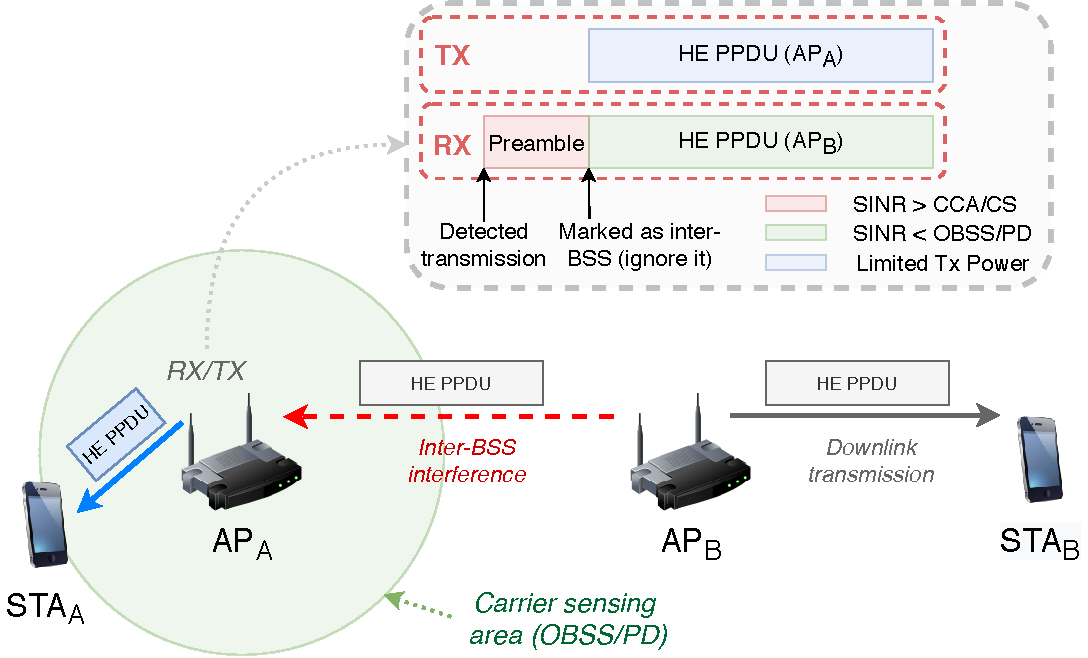
\includegraphics[width=0.8\columnwidth]{images/example_obsspd_sr}
	\caption{Example of OBSS/PD-based SR in a toy scenario.}
	\label{fig:example_obsspd_sr}
\end{figure}

% PSR 
\subsection{Parametrized Spatial Reuse}
Unlike for OBSS/PD-based SR, the PSR operation attempts to exploit triggered-based (TB) UL transmissions to carry out SR. Depending on the role of nodes participating in the PSR operation, we find two types of devices: \emph{sharing} (the ones initiating TB transmissions and indicating support for the PSR operation) and \emph{shared} (the ones taking advantage of the PSR opportunities from detected TB transmissions).

To detect PSR opportunities, shared devices must check whether their intended transmit power meets the requirements indicated in TB PPDUs from sharing devices. These requirements are based on the maximum level of interference supported by the sharing device. In particular, the minus the intended transmit power cannot exceed the following value:
\begin{equation}
\text{TX\_PWR}_{\max} = \text{TX PWR}_\text{AP} + \text{I}_\text{AP}^{\max} - RPL,
\label{eq:srp_input}
\nonumber
\end{equation}
where $\text{TX PWR}_\text{AP}$ is the normalized transmit power in dBm at the output of the antenna connector, $\text{I}_\text{AP}^{\max}$ is a normalized value in dB that captures the maximum allowed interference at the sharing device,\footnote{$\text{I}_\text{AP}^{\max}$ is computed as the target RSSI indicated in the TF minus the minimum SNR granting a 10\% PER (a safety margin is also included not to exceed 5 dB).} and Received Power Level (RPL) is measured from the legacy portion of the TF (i.e., from PHY headers).

The PSR operation is sketched in Figure \ref{fig:example_psr} for a toy scenario. As shown, the sharing device (i.e., AP$_B$) schedules an UL TB transmission by sending a TF, which is inspected by the shared device (i.e., AP$_B$) to detect a PSR-based TXOP. 
\begin{figure}[ht!]
	\centering
	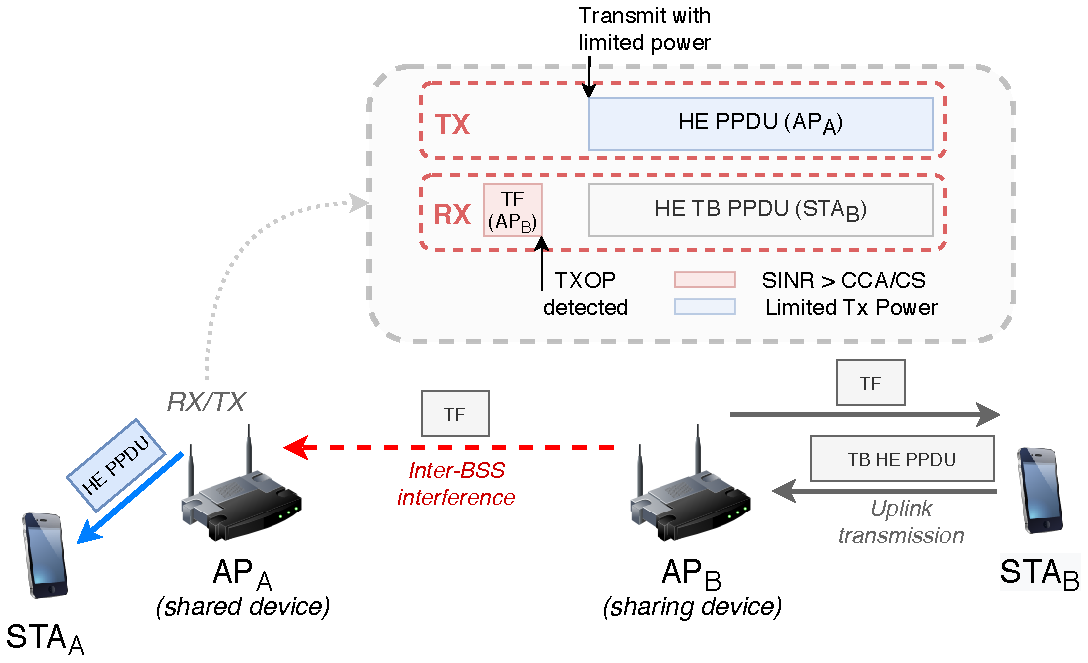
\includegraphics[width=0.8\columnwidth]{images/example_psr}
	\caption{Example of PSR in a toy scenario.}
	\label{fig:example_psr}
\end{figure}

% 11be and beyond
\section{Spatial Reuse in Future IEEE 802.11 WLANs}
Currently, the TGbe is studying a new coordinated scheme for SR. Notice that Multi-AP coordination (e.g., coordinated and joint transmission) is one of the main topics that has been so far been discussed by members of TGbe for coordinated beamforming (CBF)  \cite{tgbe_cbf}, coordinated OFDMA \cite{tgbe_cofdma}, and coordinated SR (CSR) \cite{tgbe_csr}.\footnote{Approved initial draft of PAR: \url{https://mentor.ieee.org/802.11/dcn/18/11-18-1231-01-0eht-eht-draft-proposed-par.docx}} 

Concerning CSR (or Co-SR), it aims to improve the quality of the simultaneous transmissions that can take place due to the SR operation. In particular, the transmit power of secondary transmissions take into account the maximum level of interference of the target devices to which transmissions are sought to be held. Co-SR is a natural extension of the SR scheme under the multi-AP operation framework and can be implemented with relatively low added complexity. 

% Other ways forward
Beyond 11be SR, the integration of SR with other novel mechanisms remains unexplored and it is expected to provide further performance gains. Among the most important techniques, we highlight beamforming/null steering \cite{tgbe_psr_beamforming}, OFDMA \cite{bankov2018ofdma, dovelos2018optimal}, multiple antenna systems \cite{liao2016mu}, and scheduled transmissions \cite{nurchis2019target}. For instance, the combination of SR with directional transmissions may lead to efficient and performance maximizing communications, where SR is applied on a per-beam basis. Similarly, SR can be further exploited through TB communications. In this case, users of a given BSS can be categorized into different types, so that different inter-BSS OBSS/PD values are assigned to them for the sake of scheduling joint transmissions. It is worth pointing out that users belonging to different groups can be scheduled together, provided that the most restrictive OBSS/PD threshold is used. 

% AI 
Finally, AI emerges as a potential solution to address SR because of the complexity of the problem and the characteristics of dense WLAN deployments, which are typically decentralized and highly varying in terms of users and channel dynamics. Through AI, it is possible to capture and exploit complex information that cannot be predicted on before-hand (traffic demands, user behavior, varying interference regimes, etc.). As a result, a learning-based procedure can be conducted to further improve the performance of WLAN deployments.

%%%%%%%%%%%%%%%%%
% MACHINE LEARNING
%%%%%%%%%%%%%%%%%
\chapter{Machine Learning in IEEE 802.11 WLANs}
\label{chapter3}

\section{Related Work}

\section{Multi-Armed Bandits for Decentralized Spatial Reuse}

%%%%%%%%%%%%%%%%%
% METHODS
%%%%%%%%%%%%%%%%%
\chapter{Methodology and Enablers}
\label{chapter4}

% CTMNs model
\section{Spatial Reuse through Continuous Time Markov Networks}

% 11ax OBSS/PD-based SR
\subsection{IEEE 802.11ax OBSS/PD-based Spatial Reuse}

% 11be CSR
\subsection{IEEE 802.11be Coordinated Spatial Reuse}

% Simulation
\section{System-level Simulation of Spatial Reuse}

\section{Architectural Aspects of Machine-Learning-Aware Networks}

%%%%%%%%%%%%%%%%%
% RESULTS
%%%%%%%%%%%%%%%%%
\chapter{Main Findings}
\label{chapter5}

%%%%%%%%%%%%%%%%%
% CONCLUSIONS
%%%%%%%%%%%%%%%%%
\chapter{Conclusions and Future Work}
\label{chapter6}

%%%%%%%%%%%%%%%%%
% BIBLIOGRAPHY
%%%%%%%%%%%%%%%%%
\bibliography{bibliography}

%%%%%%%%%%%%%%%%%
% ATTACHED PUBLICATIONS
%%%%%%%%%%%%%%%%%
\chapter{Publications}
\label{chapter7}

\section{Spatial Reuse in IEEE 802.11 ax WLANs}

\section{On the Performance of the Spatial Reuse Operation in IEEE 802.11 ax WLANs}

\section{Implications of decentralized Q-learning resource allocation in wireless networks}

\section{Collaborative spatial reuse in wireless networks via selfish multi-armed bandits}

\section{Potential and pitfalls of multi-armed bandits for decentralized spatial reuse in WLANs}

\section{A Flexible Machine-Learning-Aware Architecture for Future WLANs. IEEE Communications Magazine}

\section{Komondor: a wireless network simulator for next-generation high-density WLANs}

\section{Usage of Network Simulators in Machine-Learning-Assisted 5G/6G Networks}

\backmatter
\printindex

\end{document}

%NUMBER OF THE EXTERNAL PAGE EXCEPT IN THE FIRST PAGE OF EACH CAPITAL
\usepackage{fancyhdr}
\pagestyle{fancy}
\fancyfoot{}
\fancyfoot[RO]{\thepage}
\fancyfoot[LE]{\thepage}

%MULTIPLE INDEX
%In the preamble
\usepackage{multind}
\makeindex{authors}
%Introduction to form entries
\index{authors}{Einstein}
%Situation of the Index
\printindex{authors}{Author index}
%The \ usepakage {makeidx} \ makeindex \ printindex commands must be removed
%You need to exacute from the command line makeindex authors